Let $\mathcal{X}\subset\R^d$ (Borel subset) and $\norm{\cdot}$ a norm on $\R^d$. Let also $\mathcal{Y}=\{1,\cdots,K\}$ and $s:\mathcal{X}\times\mathcal{Y}\rightarrow\R$ be a measurable function (non-conformity score).

For any $x\in\mathcal{X}$ and $\epsilon \geq 0$, we set $\bouleps(x):=\left\{ \tilde{x} \in \mathcal{X} : \norm{\tilde{x} - x} \leq \epsilon\right\}$.

There are some minor measurability subtleties in the paper and the following proof, which are overlooked here for readability, but discussed in Section~\ref{sec:measurability}.

\subsection{On the continuity of $\covmax$ and $\covmin$}
\label{subsec:continuity}

\paragraph{In this section and the next}
We assume that $\CalDataset$ is fixed, so that $s(\cdot, \cdot)$ and $q_\alpha$ are deterministic. All probabilities or expectations below are taken w.r.t. the random draws of $\HoldoutDataset$ and/or $(\XYt)$. \footnote{In fact, we also work conditionally to the training set, which is treated as deterministic in all the paper.} Furthermore, since in our paper $(\CalDataset)$ is independent from $(\HoldoutDataset,(\XYt))$, all inequalities below translate into inequalities that are valid for a.e. $\CalDataset$, provided that $\mathbb{P}(\cdot)$ and $\Ex{\cdots}$ are replaced with $\mathbb{P}(\cdots | \CalDataset)$ and $\Ex{\cdots | \CalDataset}$.\\

We now study $\covmax$ and $\covmin$. For $\epsilon\geq 0$, recall that 
$$
\covmax(\epsilon) = \mathbb{P}\left(\sie(\XYt)\leq q_\alpha\right)\quad \textrm{and} \quad \covmin(\epsilon)=\mathbb{P}\left(\sse(\XYt)\leq q_\alpha\right) \;,
$$
where, in order to emphasize the dependency in $\epsilon$, we wrote
\[
\sie(x,y)=\inf\limits_{\tilde{x}\in\bouleps(x)} s(\tilde{x},y) \quad \textrm{and} \quad  \sse(x,y) = \sup\limits_{\tilde{x}\in\bouleps(x)} s(\tilde{x},y) \;.
\]

\begin{proposition}
\label{prop:continuityGamma}
    Assume that A1 and A2 from \ref{assum:X-s} hold true. Then, $\covmax$ is right-continuous on $[0,+\infty)$ and $\covmin$ is left-continuous on $(0,+\infty)$.
\end{proposition}
\begin{proof}
    We start with $\covmax$. Let $\epsilon\geq 0$ and $\eta>0$. We show that there exists $\delta>0$ s.t. $\covmax(\epsilon+\delta)\leq\covmax(\epsilon)+\eta$, which will (by monotonicity of $\covmax$) imply that $\abs{\covmax(\epsilon^\prime)-\covmax(\epsilon)}\leq \eta$ for all $\epsilon^\prime\in[\epsilon, \epsilon+\delta]$.

    Let $K\subset \mathcal{X}$ be any compact set such that $\mathbb{P}(\Xt \in K) \geq 1 - \frac{\eta}{2}$.

    By right-continuity of the cdf $t\mapsto F_\epsilon(t):=\mathbb{P}\left(\sie(\XYt)\leq t | \Xt \in K \right)$, there exists $\rho>0$ s.t. $F_\epsilon (q_\alpha + \rho) \leq F_\epsilon(q_\alpha) + \frac{\eta}{2}$.

    We now use the fact that, for each $y\in\mathcal{Y}$ (with $\mathcal{Y}$ finite), the function $s(\cdot, y)$ is continuous and thus uniformly continuous on the compact set $K_{\epsilon+1}:=\left\{ x+u : x\in K, u\in\R^d, \norm{u}\leq\epsilon+1\right\}$. Therefore, there exists $\delta\in(0,1)$ s.t., 
    \begin{equation}
        \label{eq:conti}
        \forall y \in \mathcal{Y}, \forall x, x^\prime \in K_{\epsilon+1}, \norm{x-x^\prime}\leq \delta \implies \abs{s(x,y)-s(x^\prime, y)}\leq\rho.
    \end{equation}
    Note that, for any $y\in\mathcal{Y}$ and $x\in K$, by \eqref{eq:conti} above,
    \begin{equation}
    \label{eq:sie-ineq}
        \sie(x,y)=\inf\limits_{\tilde{x}\in\bouleps(x)}s(\tilde{x},y)\leq\inf\limits_{\tilde{x}\in\boule_{\epsilon+\delta}(x)}s(\tilde{x},y)+\rho = \underline{s}_{\epsilon+\delta}(x,y)+\rho.
    \end{equation}
    \begin{figure}
        \centering
        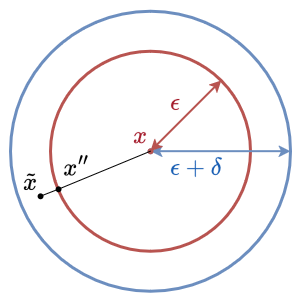
\includegraphics[width=0.3\columnwidth]{proof_illustration.png}
        \caption{Illustration of the proof of \eqref{eq:sie-ineq}. On the ball $\mathcal{B}_{\epsilon + \delta} (x)$, the score $x \mapsto s(x,y)$ is minimized at some $\Tilde{x}$. On the smaller ball $\mathcal{B}_{\epsilon}(x)$, the minimum can only be larger, but not larger than $s(x'',y)$ which is close to $s(\Tilde{x},y)$ by continuity of $s(\cdot,y)$.}
        \label{fig:preuve-2}
    \end{figure}
    This follows from Figure \ref{fig:preuve-2}. More formally, let $\tilde{x}\in\boule_{\epsilon+\delta}(x)$ be such that $s(\tilde{x},y)=\underline{s}_{\epsilon+\delta}(x,y)$. Inequality \eqref{eq:sie-ineq} is immediate if $\norm{\tilde{x}-x} \leq \epsilon$. We thus assume without loss of generality that $\norm{\tilde{x}-x}>\epsilon$. Then, let $x^{\prime\prime}\in[x,\tilde{x}] \subset\mathcal{X} $ be such that $\norm{x^{\prime\prime}-x}=\epsilon$ (recall that $\mathcal{X}$ is convex). In this case $\norm{\tilde{x}-x^{\prime\prime}}\leq\delta$ and thus (by \eqref{eq:conti}) $s(x^{\prime\prime},y)\leq s(\tilde{x}, y)+\rho$ which implies $\underline{s}_\epsilon (x,y)\leq s(x^{\prime\prime},y) \leq \underline{s}_{\epsilon+\delta}(x,y)+\rho$. This concludes the proof of \eqref{eq:sie-ineq}.

    We are ready to conclude:
    \begin{equation*}
        \begin{aligned}
        & \covmax(\epsilon+\delta)=\mathbb{P}\left(\underline{s}_{\epsilon+\delta}\left(\Xt, \Yt\right) \leq q_\alpha\right) \\
        & \leq \mathbb{P}\left(\Xt \in K\right) \cdot \mathbb{P}\left(\underline{s}_{\epsilon+\delta}\left(\Xt, \Yt\right) \leq q_\alpha \mid \Xt \in K\right)+\mathbb{P}\left(\Xt \notin K\right) \\
        & \stackrel{\text{by }\eqref{eq:sie-ineq}}{\leq} \mathbb{P}\left(\Xt \in K\right) \cdot \underbrace{\mathbb{P}\left(\underline{s}_{\epsilon}\left(\Xt, \Yt\right) \leq q_\alpha+\rho \mid \Xt \in K\right)}_{=F_{\epsilon}\left(q_\alpha+\rho\right) 
        \leq F_{\epsilon}\left(q_\alpha\right)+\frac{\eta}{2}}+\frac{\eta}{2}\\
        & \leq \mathbb{P}\left(\Xt \in K\right) \cdot\left[\mathbb{P}\left(\left.\sie\left(\Xt,\Yt\right) \leq q_\alpha \right\rvert\, \Xt \in K\right)+\frac{\eta}{2}\right]+\frac{\eta}{2} \\
        & \leq \mathbb{P}\left(\sie\left(\Xt, \Yt\right) \leq q_\alpha\right)+\eta \\
        & =\covmax(\epsilon)+\eta
        \end{aligned}
    \end{equation*}

    This entails $\abs{\covmax(\epsilon^\prime)-\covmax(\epsilon)}\leq\eta$ for all $\epsilon^\prime \in [\epsilon,\epsilon+\delta]$, and proves that $\covmax$ is right-continuous.

    The proof that $\covmin$ is left-continuous follows from similar arguments. Put briefly: for all $\epsilon>0$ and $\eta>0$, there exist a compact subset $K\subset\mathcal{X}$ and two real numbers $\rho>0$ and $\delta\in(0,\epsilon)$ such that
    \begin{equation*}
        \begin{aligned}
            & \covmin(\epsilon-\delta)=\mathbb{P}\left(\bar{s}_{\epsilon-\delta}\left(\Xt, \Yt\right) \leq q_\alpha\right) \\
        & \leq \mathbb{P}\left(\Xt \in K\right) \cdot \mathbb{P}\left(\bar{s}_{\epsilon-\delta}\left(\Xt, \Yt\right) \leq q_\alpha \mid \Xt \in K\right)+\mathbb{P}\left(\Xt \notin K\right) \\
        & \stackrel{s(\cdot,y) \text{ u.c. on } K}{\leq} \mathbb{P}\left(\Xt \in K\right) \cdot \mathbb{P}\left(\bar{s}_{\epsilon}\left(\Xt, \Yt\right) \leq q_\alpha+\rho \mid \Xt \in K\right)+\frac{\eta}{2}\\
        & \leq \mathbb{P}\left(\Xt \in K\right) \cdot\left[\mathbb{P}\left(\left.\sse\left(\Xt,\Yt\right) \leq q_\alpha \right\rvert\, \Xt \in K\right)+\frac{\eta}{2}\right]+\frac{\eta}{2} \\
        & \leq \mathbb{P}\left(\sse\left(\Xt, \Yt\right) \leq q_\alpha\right)+\eta \\
        & =\covmin(\epsilon)+\eta
        \end{aligned}
    \end{equation*}
    
    \end{proof}

    \paragraph{N.B.}
    The proof is a little easier if $s(\cdot,y)$ is uniformly continuous on $\mathcal{X}$ (e.g. if $\mathcal{X}$ is compact or $s(\cdot,y)$ is Lipschitz). In that case, there is no need to work conditionally on $\left\{\Xt \in K \right\}$.

    \subsection{Concentration of $\covmaxm$ around $\covmax$}

    Let $\HoldoutDataset=\left( X_i, Y_i \right)_{1\leq i\leq m}$ be $m\geq 2$ independent copies of $(\XYt)$.

    For $\epsilon>0$, let 
    $$
        \covmaxm(\epsilon) := \frac{1}{n} \sum\limits_{i=1}^{m}\mathds{1}_{\sie(\XYi)\leq q_\alpha}.
    $$

    Let $\delta\in(0,1)$. Since $m\covmaxm(\epsilon)\sim \mathrm{Binomial}(m,\covmax(\epsilon))$, the estimator
    $$
        \covmaxmp(\epsilon, \delta) := \max \left\{ p\in[0,1] : \mathrm{Bin}_{m,p}(m\covmaxm(\epsilon))\geq \delta\right\},
    $$
    where $\mathrm{Bin}_{m,p}$ is the c.d.f. of $\mathrm{Binomial}(m,p)$. This estimator satisfies (e.g., Theorem~3.3 by \citealt{langford2005tutorial}), for all $\epsilon \geq 0$ and $\delta\in(0,1)$,
    \begin{equation}
        \label{eq:ucb}
        \mathbb{P}\left(\covmax(\epsilon)\leq\covmaxmp(\epsilon,\delta)\right)\geq 1-\delta
    \end{equation}

    Applying \eqref{eq:ucb} $m-1$ times with properly chosen values of $\epsilon$ (of a quantile flavor), and using the fact that both $\covmax$ and $\covmaxmp(\cdot, \delta)$ are a.s. right-continuous and non-decreasing, we obtain the following ``uniform'' concentration inequality.

    \begin{theorem}
    \label{thm:appendix-thm-1}
        Assume that A1 and A2 from \ref{assum:X-s} hold true.
        Let $(\XYi)_{1\leq i \leq m}$ be $m\geq 2$ independent copies of $(\XYt)$. Then:
        $$
            \mathbb{P}\left(\forall \epsilon\geq0, \covmax(\epsilon)\leq\covmaxmp(\epsilon,\frac{\delta}{m-1})+\frac{1}{m}\right)\geq 1-\delta.
        $$
    \end{theorem}
    As seen in the proof below, $\covmax$ and $\covmaxmp(\cdot, \delta)$ are right-continuous a.s., so that the above probability is well defined (the $\forall\epsilon$ can be replaced with a countable $\forall\epsilon_k$).
    \begin{proof}
        We proceed in three steps.
        \paragraph{Step 1: right-continuity of $\covmax$ and $\covmaxmp(\cdot, \delta)$}
        \begin{itemize}
            \item the fact that $\covmax$ is right-continuous follows from Subsection \ref{subsec:continuity}.
            \item likewise, using this result with the empirical distribution $\frac{1}{m}\sum_{i=1}^{m}\delta_{(\XYi)}$, we can see that the random function $\epsilon\mapsto\covmaxm(\epsilon)$ is right-continuous, and thus locally constant to the right of any $\epsilon\geq0$. This implies that $\epsilon\mapsto\covmaxmp(\epsilon,\delta)$ is also right-continuous on $[0,+\infty)$.
        \end{itemize}

        \paragraph{Step 2: pointwise concentration and union bound}
        For every $k\in\{1,\cdots,m-1\}$, we set $\epsilon_k := \inf \left\{ \epsilon \geq 0 : \covmax(\epsilon)\geq\frac{k}{m}\right\}$, with the convention that $\inf \varnothing = +\infty$. Let also $\epsilon_m := +\infty$.
        Note that $0\leq\epsilon_1\leq \epsilon_2 \leq \cdots\leq \epsilon_m\leq +\infty$ and that $\covmax(\epsilon_k)\geq\frac{k}{m}$ whenever $\epsilon_k < \infty$ (by right-continuity of $\covmax$ on $[0,+\infty)$).
        
        First note that, if $\epsilon_1=+\infty$, then $\covmax(\epsilon)<\frac{1}{m}$ for all $\epsilon \geq 0$ by def of $\epsilon_1$). 
        In this case, the conclusion of Theorem \ref{thm:appendix-thm-1} would hold trivially.

        We can thus assume without loss of generality that $\epsilon_1<+\infty$, and set 
        $$
            K:=\max\left\{k\in\{1,\cdots,m-1\}: \epsilon_k <+\infty\right\}.
        $$
        Note that $0\leq\epsilon_1\leq\cdots\leq\epsilon_K<\epsilon_{K+1}=\cdots=\epsilon_m=+\infty$.

        Combining \eqref{eq:ucb} with a union bound, and using $K\leq m-1$, we get:

        \begin{equation}
            \label{eq:union-bound}
            \mathbb{P}\left(\forall k\in\{1,\cdots,K\}, \covmax(\epsilon_k)\leq\covmaxmp(\epsilon_k, \frac{\delta}{m-1})\right)\geq 1-\frac{K\delta}{m-1}\geq 1-\delta.
        \end{equation}

        \paragraph{Step 3: bridging the gaps}
        
        Let $\Omega_\delta := \left\{ \forall k \in \{1,\cdots,K\}, \covmax(\epsilon_k)\leq\covmaxmp(\epsilon_k, \frac{\delta}{m-1} \right\}$ be the event appearing in \eqref{eq:union-bound}. 
        We now work on the event $\Omega_\delta$.

        Let $\epsilon\geq\epsilon_1$. Note that $\epsilon$ belongs to one of the following K disjoint (possibly empty) intervals:
        $$
            I_k = [\epsilon_k, \epsilon_{k+1}), k\in\{1,\cdots,K\} \quad \text{(by convention, $I_k=\varnothing$ if $\epsilon_k=\epsilon_{k+1}$)}.
        $$
        We let $k\in\{1,\cdots,K\}$ be such that $\epsilon\in I_k$, i.e., $\epsilon_k \leq \epsilon < \epsilon_{k+1}$.

        Recall that $\covmax(\epsilon_k)\geq\frac{k}{m}$, and note that $\covmax(\epsilon)\leq\frac{k+1}{m}$. 

        Therefore,
        \begin{equation*}
            \begin{aligned}
                \covmax(\epsilon) &\leq \frac{k+1}{m}\\
                &\leq \covmax(\epsilon_k) + \frac{1}{m}\\
                &\leq \covmaxmp(\epsilon_k,\frac{\delta}{m-1})+\frac{1}{m} & \text{(we work on $\Omega_\delta$)}\\
                &\leq \covmaxmp(\epsilon, \frac{\delta}{m-1})+\frac{1}{m} &\text{(by $\epsilon_k \leq \epsilon$ and monotonicity of $\covmaxmp(\cdot,\frac{\delta}{m-1}))$}
            \end{aligned}
        \end{equation*}

        Since we also have $\covmax(\epsilon)\leq\frac{1}{m}$ if $\epsilon_1>0$ and $\epsilon \in [0,\epsilon_1)$ (by definition of $\epsilon_1$), we just proved that, on the event $\Omega_\delta$,
        $$
            \forall \epsilon \geq 0, \covmax(\epsilon) \leq \covmaxmp(\epsilon, \frac{\delta}{m-1})+\frac{1}{m}.
        $$
        Recalling that $\mathbb{P}(\Omega_\delta)\geq 1-\delta$ concludes the proof.
    \end{proof}

    We can control $\covmin=\mathbb{P}(\sse(\XYt)\leq q_\alpha)$ similarly (up to a coin flip), using
    $$
        \covminm := \frac{1}{m}\sum\limits_{i=1}^{m}\mathds{1}_{\sse(\XYi) \leq q_\alpha}
    $$
    and
    $$
        \covminmm(\epsilon,\delta) := 1-\max\left\{p\in[0,1] : \mathrm{Bin}_{m,p}(m(1-\covminm(\epsilon)))\geq\delta\right\}.
    $$
    We have the following lower bound.


    %%%%%% THOMAS BELOW HERE %%%%%%%%%%

    \begin{theorem}
    \label{thm:appendix-thm-2}
        Assume that A1 and A2 from \ref{assum:X-s} hold true. Let $(\XYi)_{1\leq i \leq m}$ be $m\geq2$ independent copies of $(\XYt)$. Then:

        \begin{equation}
            \mathbb{P}\left(\forall \epsilon > 0, \covmin(\epsilon) \geq \covminmm\left(\epsilon, \frac{\delta}{m-1}\right)-\frac{1}{m}\right) \geq 1-\delta.
        \end{equation}
    \end{theorem}

    % \begin{remark}
    %     The case $\epsilon=0$ is not guaranteed, it would be with $\frac{\delta}{m}$ instead of $\frac{\delta}{m-1}$.
    % \end{remark}

    First, note that our high probability lower bound on $\covmin(\epsilon)$ is similar to our high probability upper bound on $\covmax(\epsilon)$, by a simple coin flip. Indeed, note that:

    \begin{equation}
    \begin{aligned}
        1 - \covmin(\epsilon) &= \mathbb{P}\left(\sse(\XYt) > q_\alpha\right). \\
        1 - \covminm(\epsilon) :&= \frac{1}{m}\sum\limits_{i=1}^m \mathds{1}_{\sse(\XYi) > q_\alpha} \\
        1 - \covminmm(\epsilon, \delta) :&= \max\{ p \in [0,1]: \mathrm{Bin}_{m,p}\left( m \cdot (1 - \covmin(\epsilon))\right) \geq \delta \}
    \end{aligned}
    \end{equation}

    \paragraph{Issue} Though these functions are non-decreasing in $\epsilon$, they are \textit{left}-continuous. This calls for additional technicalities, as seen in the proof below.

    \begin{proof}
    We also proceed with three steps: many arguments are identical, but not all.

    \paragraph{Step 1: left continuity of $\covmin$ and $\covminmm(\cdot, \delta)$ on $(0,+\infty)$} This follows from similar arguments as in the proof of Theorem~\ref{thm:appendix-thm-1}.

    \paragraph{Step 2: Pointwise concentration and union bound}
    For every $k \in \{1,\cdots,m-1\}$, we set $\epsilon_k := \inf \{ \epsilon \geq 0 : 1 - \covmin(\epsilon) \geq \frac{k}{m}\}$, with the convention that $\inf \varnothing = + \infty$. Let also $\epsilon_m := + \infty$.
    
    Note that $0 \leq \epsilon_1 \leq \epsilon_2 \leq \cdots \leq \epsilon_m \leq +\infty$ and that $1-\covmin(\epsilon_k) \leq \frac{k}{m}$ whenever $0 < \epsilon_k \leq +\infty$ (by left continuity of $\covmin$ on $(0,+\infty)$).

    First note that, if $\epsilon_1=+\infty$, then $\covmin(\epsilon) > 1 - \frac{1}{m}$ for all $\epsilon \geq 0$ (by def of $\epsilon_1)$. In this case, the conclusion of Theorem~\ref{thm:appendix-thm-2} would hold trivially.

    We can thus assume without loss of generality that $\epsilon_1 < +\infty$, and set 

    $$
        K:= \max\left\{k\in\{1,\cdots,m-1\}: \epsilon_k < +\infty \right\}.
    $$

    Note that $0 \leq \epsilon_1 \leq \cdots \leq \epsilon_K \leq \epsilon_{K+1} = \cdots = \epsilon_m = + \infty$.

    We now need additional technicalities.

    For any $q \in \mathbb{N}^* = \{1, 2, \cdots\}$ and $k \in \{1,\cdots,K\}$, we set

    \begin{equation*}
        \epsilon_k^q = \begin{cases}
            \left(1-\frac{1}{q}\right) \epsilon_k + \frac{1}{q}\epsilon_{k+1} & \text{if} \ k \leq K-1 \\
            \epsilon_k + \frac{1}{q} & \text{if} \ k = K
        \end{cases}
    \end{equation*}

    Note that 
    \begin{equation*}
        \begin{cases}
            \epsilon_k < \epsilon_k^q < \epsilon_{k+1} & \text{if} \ \epsilon_k < \epsilon_{k+1}. \\
            \epsilon_k = \epsilon_k^q = \epsilon_{k+1} & \text{if} \ \epsilon_k = \epsilon_{k+1}.
        \end{cases}
    \end{equation*}

    and that $\epsilon_k^{q+1} \leq \epsilon_k^q$. 


    By Langford (2005, Theorem 3.3), we have similarly  to \eqref{eq:ucb},
    \begin{equation}
    \label{eq:ucb-min}
        \forall \epsilon \geq 0, \forall \delta \in (0,1), \mathbb{P}\left(\covmin(\epsilon)\geq \covminmm(\epsilon,\delta)\right)\geq 1-\delta.
    \end{equation}
        
    Let $\delta\in(0,1)$. Combining \eqref{eq:ucb-min} with a union bound, we get, for any $q\geq 1$,

    \begin{equation}
        \label{eq:uni-min}
        \mathbb{P}\left( \forall k \in \{ 1,\cdots, K\}, \covmin(\epsilon^q_k) \geq \covminmm(\epsilon_k^q,\frac{\delta}{m-1})\right)\geq 1-\delta.
    \end{equation}
    We now work on the event 
    $$
        \Omega_\delta^q := \left\{ \forall k \in \{ 1,\cdots, K \}, \covmin(\epsilon_k^q)\geq \covminmm(\epsilon^q_k, \frac{\delta}{m-1})\right\}.
    $$
    We set $\Epsilon^q := \left( \bigcup_{k=1}^{K-1} (\epsilon_q^k, \epsilon_{k+1}] \right) \cup (\epsilon_K^q, +\infty)$,
    where $(\epsilon^q_k,\epsilon_{k+1}]=\varnothing$ if $\epsilon_k = \epsilon_{k+1}$.
    Note that $\Epsilon^q \subseteq \Epsilon^{q+1} \subseteq (\epsilon_1, +\infty)$ and $\cup_{q\geq 1}\Epsilon^q = (\epsilon_1, +\infty)$

    Now, let $\epsilon \in \Epsilon^q$. There exists $k\in\{1,\cdots,K\}$ such that $k\leq K-1$ and $\epsilon \in (\epsilon_k^q, \epsilon_{k+1}]$, or $k=K$ and $\epsilon\in(\epsilon^q_K, +\infty)$. In particular, $\epsilon_k < \epsilon_k^q$ whatever the value of k.

    Note that, if $k \leq K-1$, we have $0<\epsilon_{k+1}<+\infty$ and therefore $1-\covmin(\epsilon_{k+1})\leq\frac{k+1}{m}$.
    This entails (using $\epsilon\leq\epsilon_{k+1}$ and the fact that $1-\covmin$ is non-decreasing)
    $$
        1-\covmin(\epsilon)\leq\frac{k+1}{m},
    $$
    which is also true $k=K$ (by def of $\epsilon_{K+1}$ if $K+1\leq m-1$, or trivial if $K=m=1$).
    Therefore, whatever the value of $k$ above,

    \begin{equation}
        \begin{aligned}
            1 - \covmin(\epsilon) &\leq \frac{k+1}{m} \\
            &\leq 1 - \covmin(\epsilon_k^q)+\frac{1}{m} &\text{(since } 1 - \covmin(\epsilon_k^q) \geq \frac{k}{m}, \text{ by def of $\epsilon_k$ and $\epsilon_k^q > \epsilon_k)$} \\
            &\leq 1 - \covminmm(\epsilon_k^q,\frac{\delta}{m-1}) + \frac{1}{m} & \text{(we work on $\Omega_{\delta}^{q}$)} \\
            &\leq 1 - \covminmm(\epsilon,\frac{\delta}{m-1}) + \frac{1}{m} & \text{(by $\epsilon_k^q \leq \epsilon$ and monotonicity of $\covminmm(\cdot,\frac{\delta}{m-1})$)}\\
        \end{aligned}
    \end{equation}

    Rearranging terms, we proved that, on the event $\Omega_{\delta}^q$,

    \begin{equation}
        \forall \epsilon \in \Epsilon^q, \covmin(\epsilon) \geq \covminmm(\epsilon,\frac{\delta}{m-1}) - \frac{1}{m}.
    \end{equation}


    We now let $q\rightarrow+\infty$. More precisely, recalling that $(\epsilon_1, +\infty)=\cup_{q\geq 1} \Epsilon^q$,

    \begin{equation*}
        \begin{aligned}
            \mathbb{P}&\left(\forall \epsilon \in (\epsilon_1, +\infty), \covmin(\epsilon) \geq \covminmm(\epsilon, \frac{\delta}{m-1})-\frac{1}{m}\right)\\
            &=\mathbb{P}\left(\cap_{q \geq 1} \{\forall \epsilon \in \Epsilon^q, \covmin(\epsilon) \geq \covminmm(\epsilon, \frac{\delta}{m-1})-\frac{1}{m}\}\right)\\
            &=\lim\limits_{q\rightarrow +\infty} \mathbb{P}\left(\forall \epsilon \in \Epsilon^q, \covmin(\epsilon) \geq \covminmm(\epsilon,\frac{\delta}{m-1})-\frac{1}{m}\right) & \text{(since $\Epsilon^q \subseteq \Epsilon^{q+1}$)}\\
            &\geq 1-\delta. & \text{(since $\mathbb{P}(\Omega_\delta^q)\geq 1-\delta$)}
        \end{aligned}
    \end{equation*}
    Nothing that, if $\epsilon_1 > 0$, then $1-\covmin(\epsilon) \leq \frac{1}{m}$ for all $\epsilon \in [0,\epsilon_1]$, concludes the proof.   
\end{proof}


